\documentclass[twoside=semi,fontsize=12pt,paper=a4,titlepage=on]{kv_article}
%\documentclass[twoside=true,fontsize=12pt,paper=a4,titlepage=off]{article}
\usepackage{graphicx}
\usepackage{amssymb, amsmath, bm}
\usepackage{multirow}
\usepackage{mathtools}
\usepackage{array}
\usepackage{enumitem}
\usepackage{arydshln}
\usepackage{subfig}
\usepackage{tabularx}

\begin{document}

\title{Impact of elevation angle on weighted baseline length repeatability}
\subtitle{\vspace{1cm}Case study: Local baselines in Ny-Ålesund and Wettzell}
%{\vspace{2cm}Norwegian Mapping Authority}
\author{Ann-Silje Kirkvik}
\date{\today}

\maketitle

\section{Background}
NYALE13S started observing in February 2020 with a triband receiver and NYALES20 stopped observing in July 2023. The NYALES20 antenna have been dismantled after almost 30 years of operations. The two stations have observed in parallel for almost 3 years to help connect the new VGOS network with the legacy S/X network. The NYALE13S antenna will eventually switch to a VGOS receiver. In addition, NYALE13N started observing in August 2022 with a VGOS receiver.

The baseline length repeatability of the NYALE13S/NYALES20 baseline have been higher than the similar baseline in Germany between WETTZELL and WETTZ13N \cite{kirkvik2021}. NYALES20 and WETTZELL are both old 20-meter antennas that have participated in many global sessions and are regularly contributing to the determination of earth orientation parameters and the international terrestrial reference frame. Like NYALE13S, WETTZ13N is a 13-meter antenna with a legacy receiver (S/X) that has observed many session together with the local 20-meter antenna. There is also a third station, WETTZ13S, in Germany with a VGOS receiver.

\sloppy
The NYALES20/NYALE13S baseline is approximately 1540 meters and the WETTZELL/WETTZ13N baseline is approximately 120 meters. The German baseline is shorter than the Norwegian one, but in a VLBI context where baselines usually are intercontinental, both these baselines are short. This study investigates one potential candidate for the different performance of the two baselines.

\fussy
In GNSS, there is the concept of Position Dilution Of Precision (PDOP). This parameter says something about the expected precision of a position based on the satellite geometry. A good spread of satellites in the sky yields a better PDOP value. It is therefore desirable to have many satellites at different elevation and azimuth angles. Similarly, in VLBI it is desirable to have many observations to radio sources at different positions in the sky. In addition, the data from satellites and radio sources at low elevation angles have a longer travel path through the troposphere and therefore provide useful information about the troposphere. In both GNSS and VLBI analysis, the troposphere needs to be estimated to be able to remove the effect of the troposphere on the signal path. The theory is then that the observations at low elevation angles are especially valuable to the data analysis. This has been studied and verified already. See for instance \cite{teke2008}. % https://ivscc.gsfc.nasa.gov/publications/gm2008/teke.pdf == https://yunus.hacettepe.edu.tr/~kteke/index_files/proceedings/Teke_etal_2008_5th_IVS_paper.pdf

The new observatory in Ny-Ålesund is build lower in the terrain than the old observatory and it is closer to the sea. The radar from the boats that enter the harbor in Ny-Ålesund is a threat to the sensitive equipment in the antennas. In the NYALE13S antenna the X-band low noise amplifier (LNA) have been destroyed on multiple occasions due to the boat radars \cite{perez2019}. To mitigate this effect the antennas at the new observatory should never point towards the sea with an elevation angle lower than 15$^\circ$. As a consequence, the elevation masks have been set to 15$^\circ$ regardless of azimuth angle. Can this be one of the reasons for the higher baseline repeatability results in Ny-Ålesund and should the elevation mask be refined?

\section{Data and Method}
\label{sec:data_and_method}
This analysis includes all global 24 hour sessions from 2020-01-01 to 2024-04-01 where either of the stations in Ny-Ålesund participated. Since NYALES20 and WETTZELL regularly participate in these sessions it gives a decent amount of sessions to work with. The WETTZELL/WETTZ13N baseline have a longer history and more data from this site could be included, but this baseline already performs better than the NYALES20/NYALE13S baseline on the data selected based on participation from Ny-Ålesund. There are also some sessions with the baselines NYALES20/NYALE13N, NYALE13N/NYALE13S, WETTZELL/WETTZ13S and WETTZ13S/WETTZ13N but not enough for a useful comparison. This study therefore focuses on comparing the NYALES20/NYALE13S and WETTZELL/WETTZ13N baselines. 

The data analysis is performed using Where\footnote{https://kartverket.github.io/where} \cite{hjelle2018}. The analysis strategy is the same that is used when analyzing regular R1/R4 sessions. That means that station coordinates, source coordinates and all earth orientation parameters are estimated. The station and source coordinates are solved by applying NNT/NNR constraints to ITRF2020 and NNR to ICRF3, respectively. In addition, clock and troposphere parameters are estimated. For more information see \cite{kirkvik2017b} and \cite{kirkvik2019}. By default no observations are discarded based on the elevation angle; the default elevation angle cut off is 0$^\circ$. However, observations are rarely scheduled below 5$^\circ$.

To test the impact of low observations at elevation angles a second analysis was done with the elevation angle cut off set to 15$^\circ$. This cut off was applied to all stations in a session, not just the German and Norwegian stations. On average, this will discard 20\% of the observations and the natural consequence of having fewer observations is to get higher formal errors for the computed station coordinates and the baseline length. Therefore, a third analysis was also conducted. Instead of discarding observations with low elevation angles, approximately 20\% of the observations where discarded from each session at random. The second and third analysis should therefore, on average, be based on the same amount of observations, but with different distributions of the observations in the sky.

The weighted baseline length and weighted baseline repeatability is calculated according to \cite{hofmeister2016}. The baselines are also compared to the measured local ties. See \cite{tangen2021} and \cite{schuler2018}.

\section{Results}
In this study the data is analyzed with three different scenarios as described in \ref{sec:data_and_method}. Figure \ref{fig:sky}, \ref{fig:sky15} and \ref{fig:sky_random} shows the accumulated azimuth and elevation angles for all observations in all sessions in the three scenarios. NYALES20 is to some extent blocked by mountains in the south and west, but still have a significant number of observations at low elevation angles. As expected NYALE13S has very limited number of observations below 15$^\circ$ elevation. All the observations with elevation angle below 15$^\circ$ for NYALE13S are from 2020 and the total amount is 563 observations across 18 sessions. Discarding observations randomly seem to mostly preserves the sky distribution of the observations.


%Elevation below 15 degrees for 54 obs for NYALE13S in session 2020-02-17 r1934
%Elevation below 15 degrees for 27 obs for NYALE13S in session 2020-02-24 r1935
%Elevation below 15 degrees for 9 obs for NYALE13S in session 2020-03-02 r1936
%Elevation below 15 degrees for 25 obs for NYALE13S in session 2020-03-09 r1937
%Elevation below 15 degrees for 21 obs for NYALE13S in session 2020-03-23 r1939
%Elevation below 15 degrees for 12 obs for NYALE13S in session 2020-03-30 r1940
%Elevation below 15 degrees for 7 obs for NYALE13S in session 2020-04-27 r1944
%Elevation below 15 degrees for 12 obs for NYALE13S in session 2020-05-04 r1945
%Elevation below 15 degrees for 3 obs for NYALE13S in session 2020-05-11 r1946
%Elevation below 15 degrees for 88 obs for NYALE13S in session 2020-05-18 r1947
%Elevation below 15 degrees for 54 obs for NYALE13S in session 2020-05-26 r1948
%Elevation below 15 degrees for 8 obs for NYALE13S in session 2020-06-02 r1949
%Elevation below 15 degrees for 24 obs for NYALE13S in session 2020-06-15 r1951
%Elevation below 15 degrees for 46 obs for NYALE13S in session 2020-06-22 r1952
%Elevation below 15 degrees for 69 obs for NYALE13S in session 2020-11-03 r1971
%Elevation below 15 degrees for 56 obs for NYALE13S in session 2020-11-30 r1975
%Elevation below 15 degrees for 27 obs for NYALE13S in session 2020-12-22 r4978
%Elevation below 15 degrees for 21 obs for NYALE13S in session 2020-12-29 r4979
% Total: [54,27,9 ,25,21,12,7 ,12,3 ,88,54,8 ,24,46,69,56,27,21] = 563

NYALES20 seem to have more observations with higher residuals than WETTZELL. In this study NYALES20 observed past its originally planned end of life and had a lot of different technical problems. Both 13-meter antennas (NYALE13S and WETTZ13N) also have more of the higher residuals, but these antennas are designed to work with a broadband VGOS receiver and not a legacy S/X receiver. There is therefore nothing unexpected to see in the colors of the sky plots.

Figure \ref{fig:bl_nsny} and \ref{fig:bl_wzwn} and table \ref{tab:baselines} show the weighted baseline length repeatability and the weighted baseline length for the two baselines and the three scenarios. The baseline plots all have the same scale on the y-axis; there are 20 mm from top to bottom and 2.5 mm between each dotted gray line. As expected the baseline length repeatability becomes higher when observations at low elevation angles are discarded. It also becomes higher when 20\% of the observations are discarded, but not as high as when the low elevation observations are discarded. This confirms that the number of observations are important to get good results, but, more importantly, that the observations at low elevation angles are have a high impact on the performance of the baseline. In earlier studies of the NYALE13S/NYALES20 baseline (\cite{kirkvik2021}) the offset between the weighted baseline length and the local tie measurement was 0.0000 meters. This analysis was done with data mostly from 2020, which included some observations for NYALE13S at low elevation angles. As more sessions where observed and included in the analysis the offset grew and the baseline length repeatability did not improve. Missing observations on low elevation angles from 2021 and onward seems like a plausible explanation for this lack of improvement and worsening of the offset. 

Table \ref{tab:num_obs} shows the number of observations used in total for all stations and for the four stations WETTZELL, WETTZ13N, NYALE13S and NYALES20. Since NYALE13S already have very limited number of observations below 15$^\circ$ elevation, this station only lose 11\% of the observations in the second scenario. Therefore, the third scenario might degrade the solution for this station more than the other stations. Regardless, the second scenario is the worst scenario also for the the NYALES20/NYALE13S baseline. 

Comparing the weighted baseline length with the local tie shows the same behavior. The difference is larger with fewer observations but largest when observations at low elevation angles are discarded. The observations at low elevation angle is important to determine the station height and missing these observations clearly have an impact on the computed baseline length. 

 
\begin{figure}
\centering
    % Sky plot NYALES20 - cut off 0 degrees
	\subfloat[\textcolor{black}{NYALES20}.\label{fig:sky-1}]
      {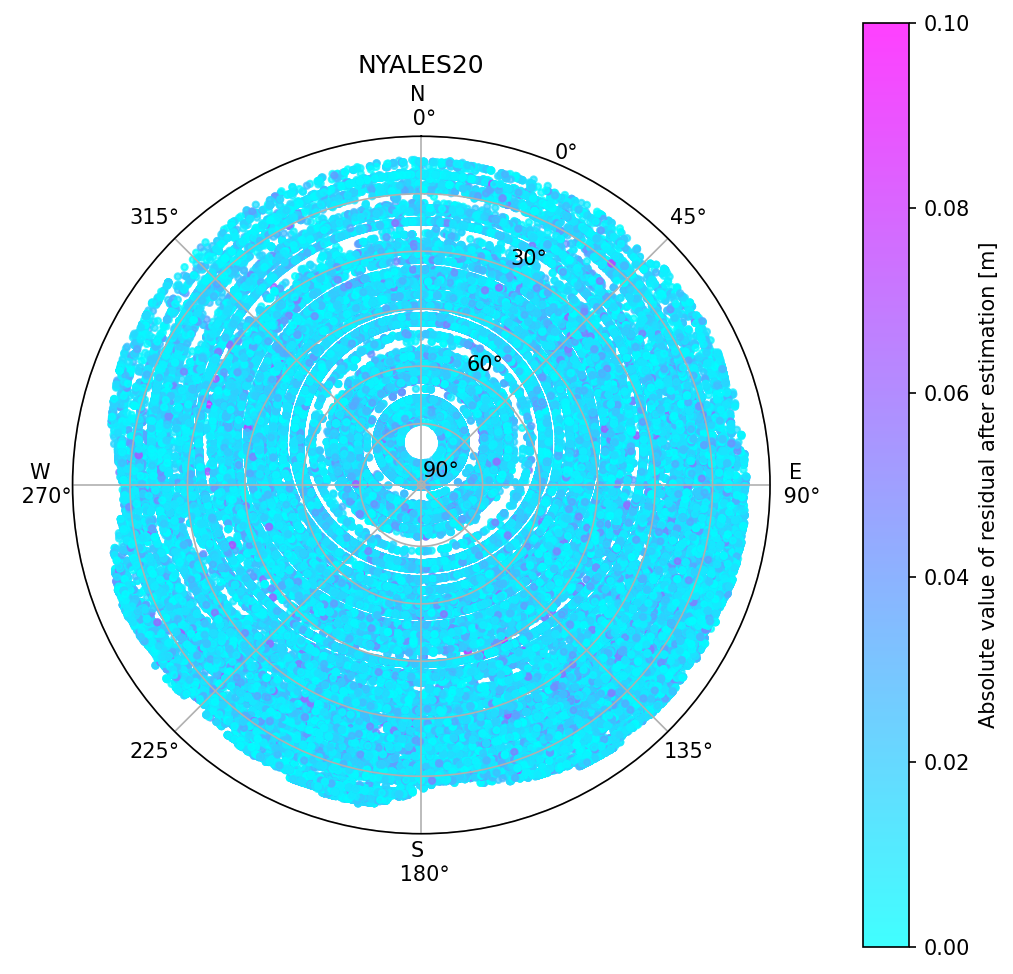
\includegraphics[width=0.5\linewidth]{fig/Skyplot_NYALES20_2020-01-01_2024-04-01_nyales}} %\\
    % Sky plot NYALE13S - cut off 0 degrees
	\subfloat[\textcolor{black}{NYALE13S}.\label{fig:sky-2}]
      {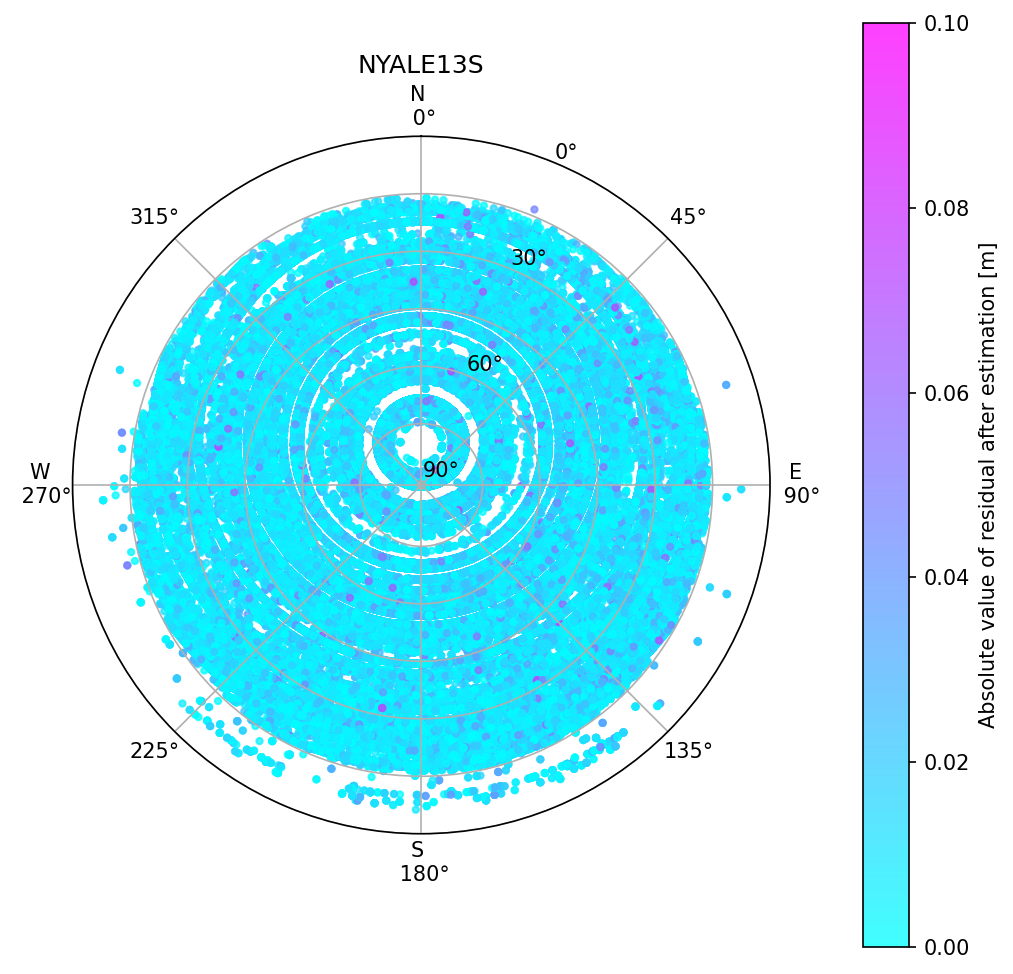
\includegraphics[width=0.5\linewidth]{fig/Skyplot_NYALE13S_2020-01-01_2024-04-01_nyales}} \\
    % Sky plot WETTZELL - cut off 0 degrees
	\subfloat[\textcolor{black}{WETTZELL}.\label{fig:sky-3}]
      {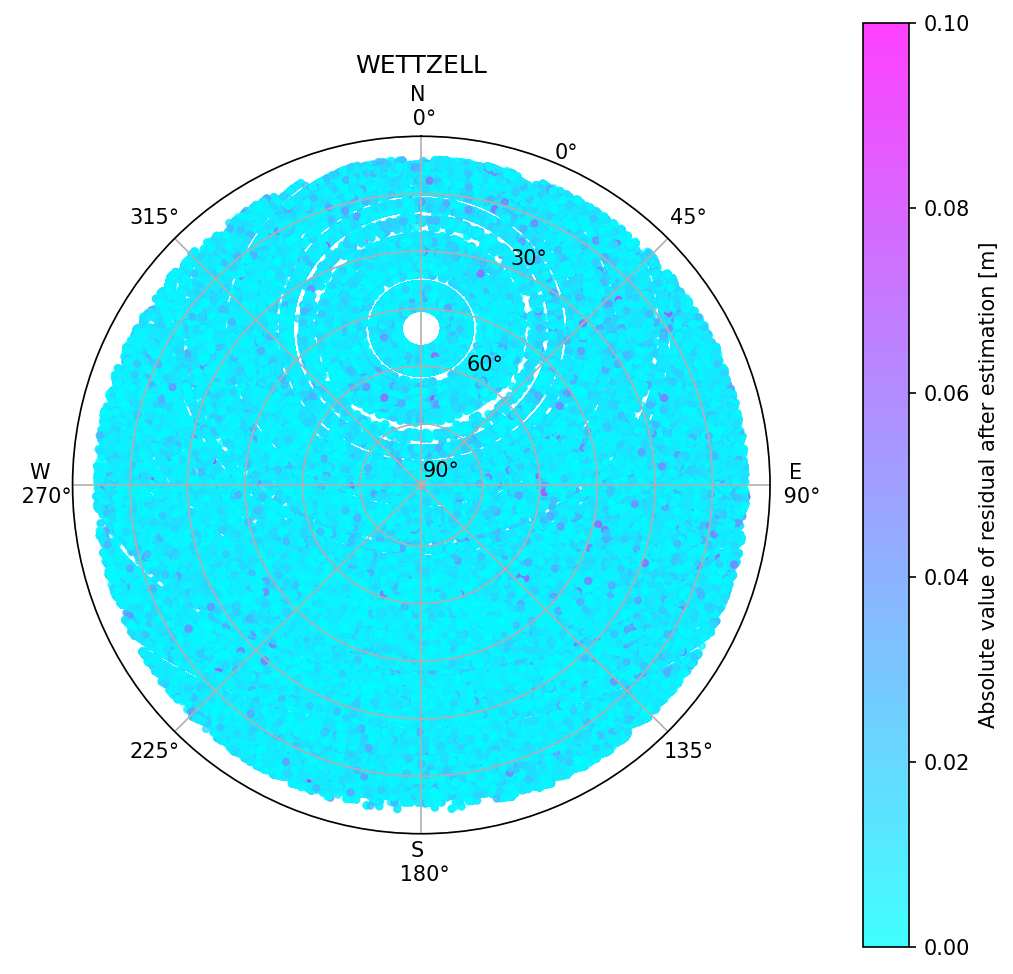
\includegraphics[width=0.5\linewidth]{fig/Skyplot_WETTZELL_2020-01-01_2024-04-01_nyales}} %\\
    % Sky plot WETTZ13N - cut off 0 degrees
	\subfloat[\textcolor{black}{WETTZ13N}.\label{fig:sky-4}]
      {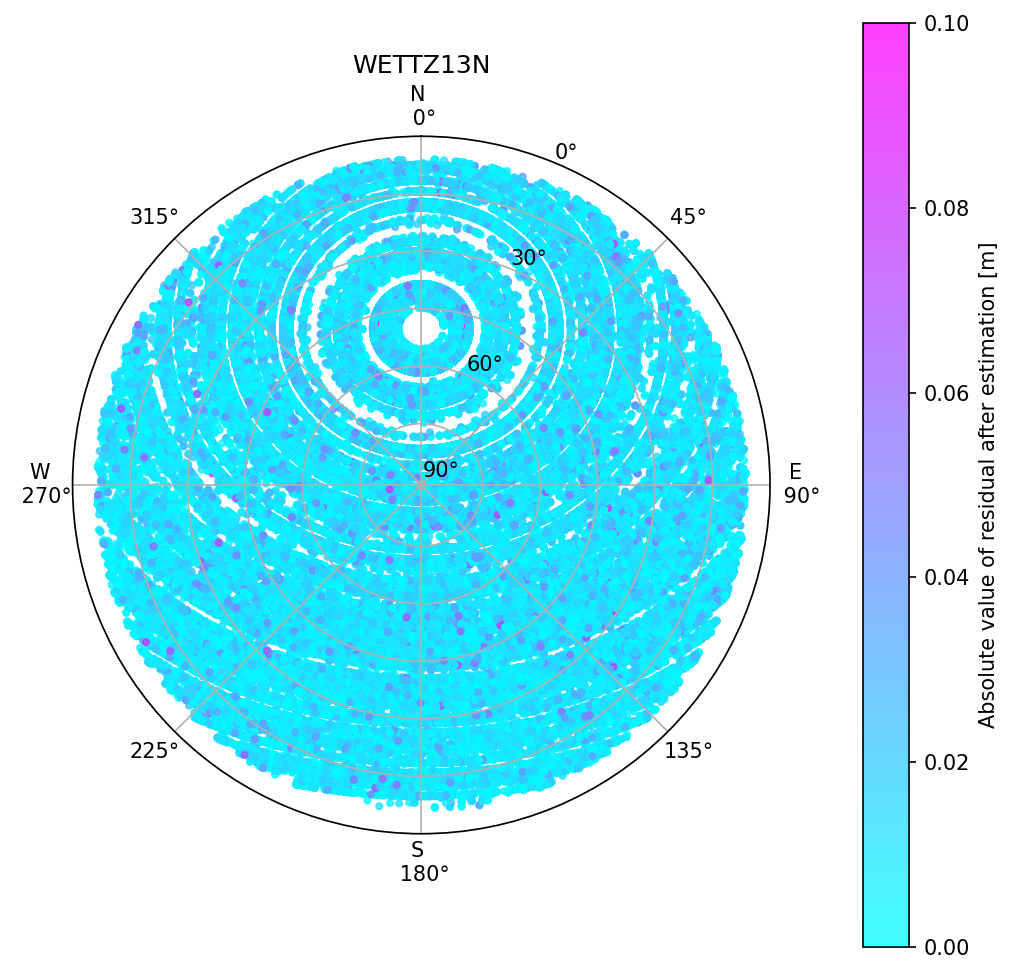
\includegraphics[width=0.5\linewidth]{fig/Skyplot_WETTZ13N_2020-01-01_2024-04-01_nyales}} \\
    \caption{Accumulated sky plots of the four stations NYALES20 (\ref{fig:sky-1}), NYALE13S (\ref{fig:sky-2}), WETTZELL (\ref{fig:sky-3}) and WETTZ13N (\ref{fig:sky-4}) with an elevation cut off angle of 0$^\circ$. The color represents the residual of each observation after estimation. Darker color means higher residuals. The colors may be useful to see if there is a problem in any particular direction.}
	\label{fig:sky}
\end{figure}

\begin{figure}
\centering
    % Sky plot NYALES20 - cut off 15 degrees
	\subfloat[\textcolor{black}{NYALES20}.\label{fig:sky15-1}]
      {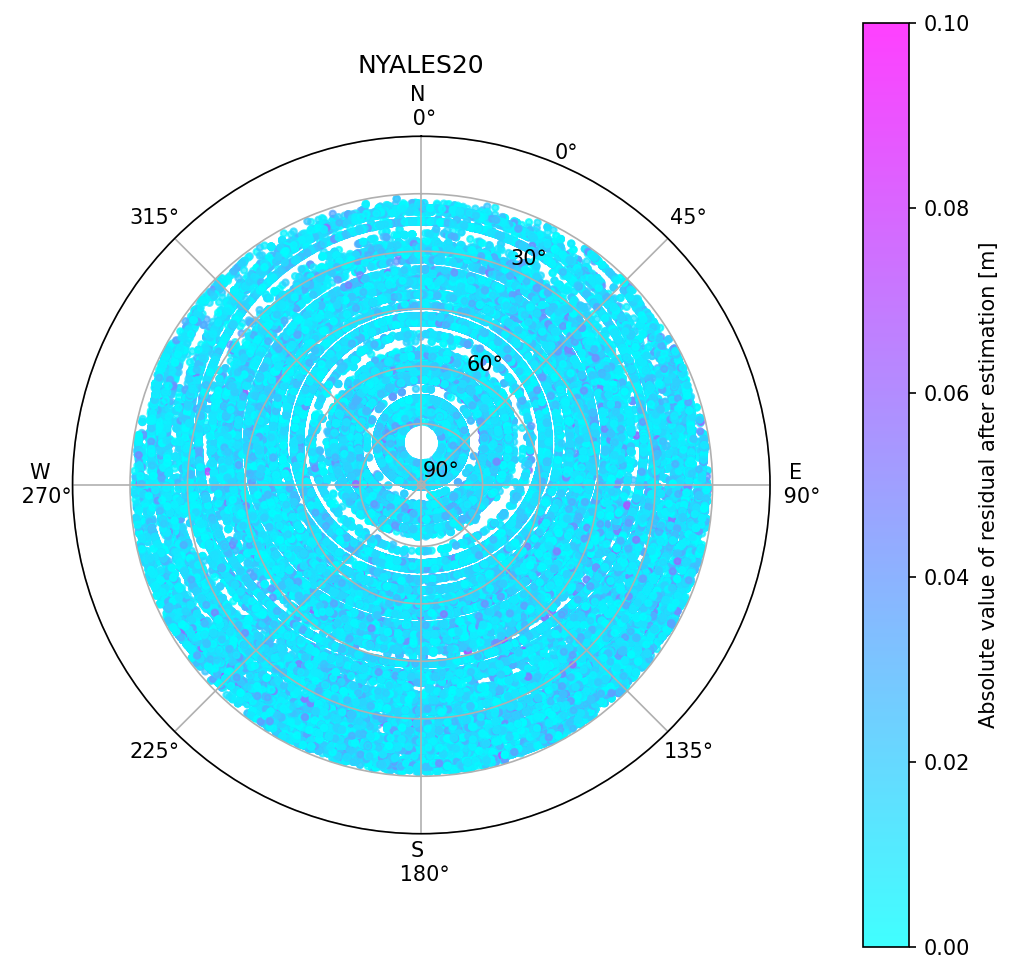
\includegraphics[width=0.5\linewidth]{fig/Skyplot_NYALES20_2020-01-01_2024-04-01_elev15}} %\\
    % Sky plot NYALE13S - cut off 15 degrees
	\subfloat[\textcolor{black}{NYALE13S}.\label{fig:sky15-2}]
      {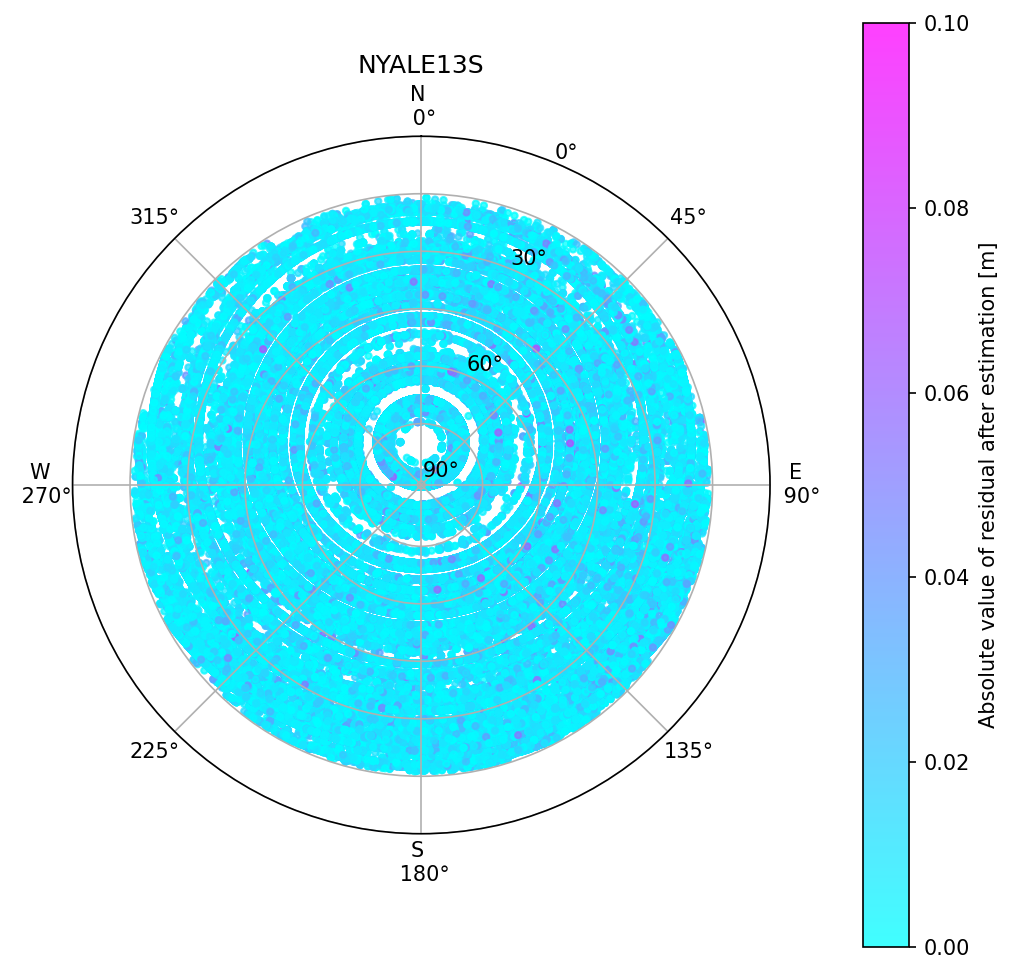
\includegraphics[width=0.5\linewidth]{fig/Skyplot_NYALE13S_2020-01-01_2024-04-01_elev15}} \\
    % Sky plot WETTZELL - cut off 15 degrees
	\subfloat[\textcolor{black}{WETTZELL}.\label{fig:sky15-3}]
      {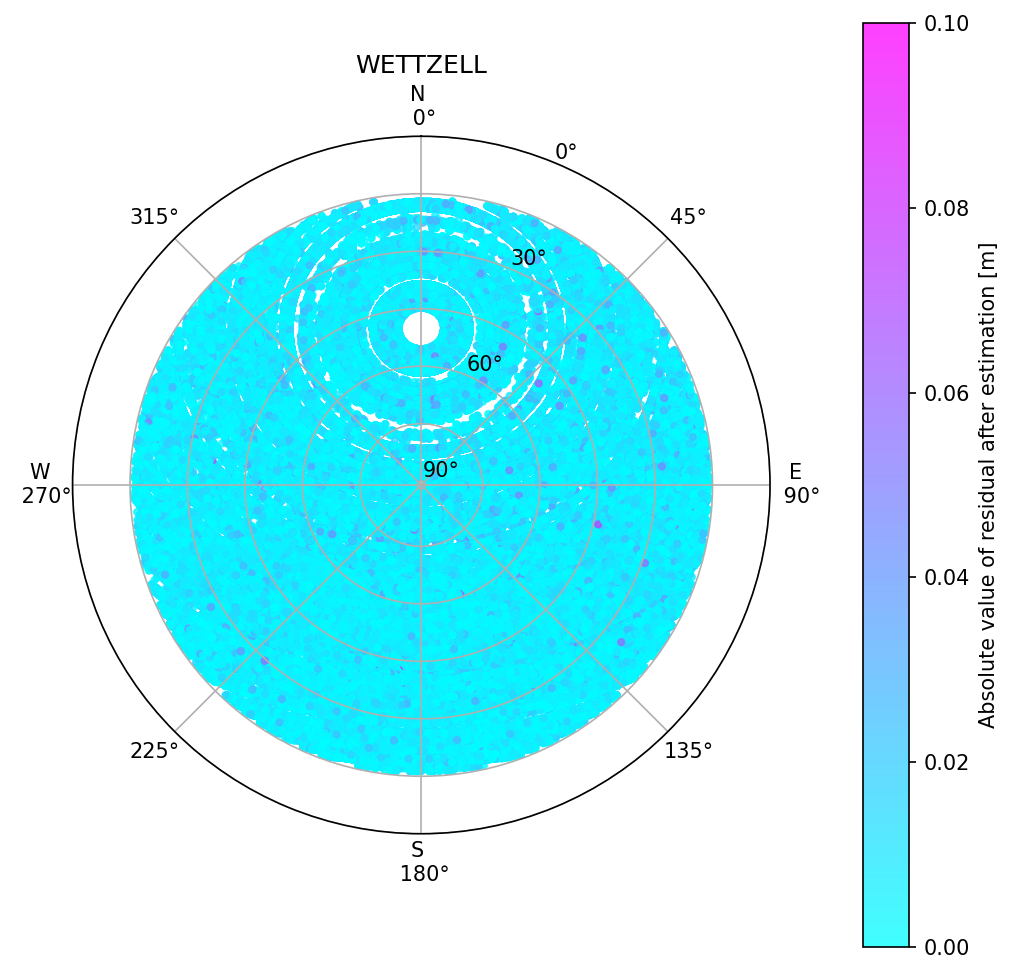
\includegraphics[width=0.5\linewidth]{fig/Skyplot_WETTZELL_2020-01-01_2024-04-01_elev15}} %\\
    % Sky plot WETTZ13N - cut off 15 degrees
	\subfloat[\textcolor{black}{WETTZ13N}.\label{fig:sky15-4}]
      {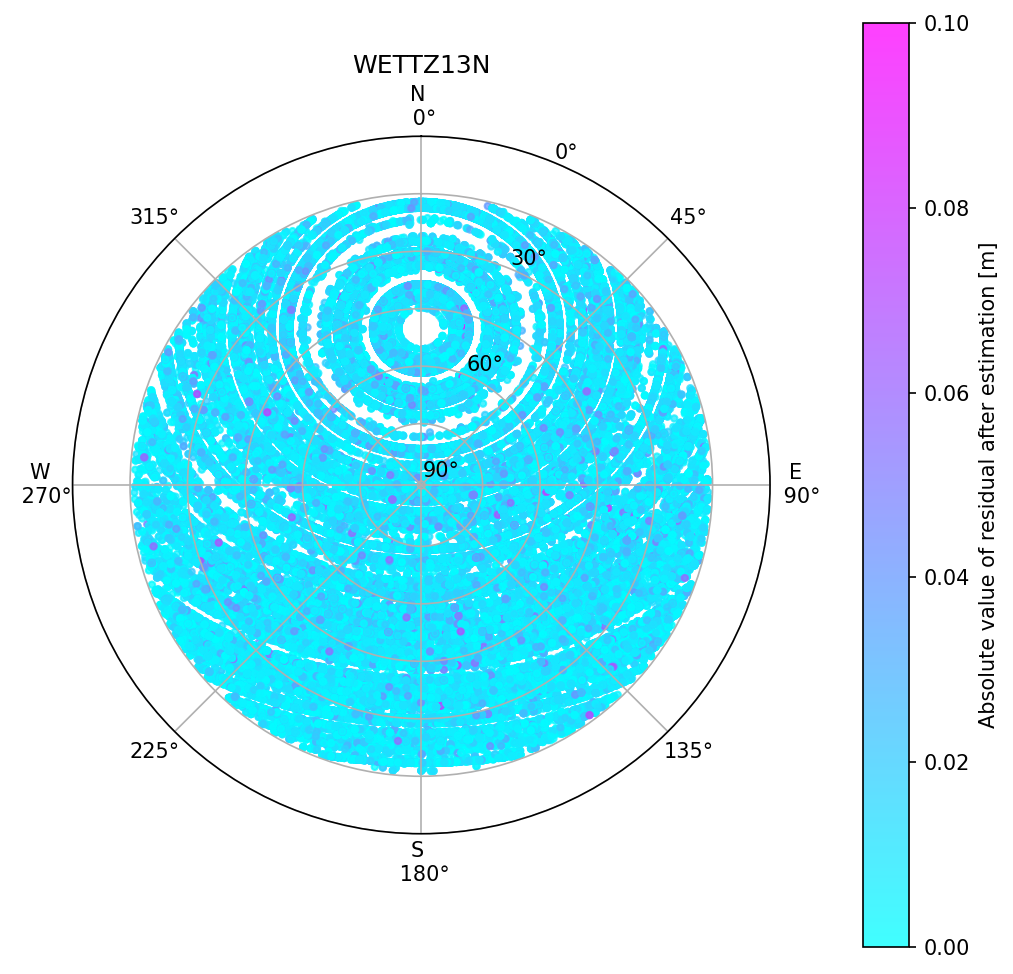
\includegraphics[width=0.5\linewidth]{fig/Skyplot_WETTZ13N_2020-01-01_2024-04-01_elev15}} \\
    \caption{Accumulated sky plots of the four stations NYALES20 (\ref{fig:sky15-1}), NYALE13S (\ref{fig:sky15-2}), WETTZELL (\ref{fig:sky15-3}) and WETTZ13N (\ref{fig:sky15-4}) with an elevation cut off angle of 15$^\circ$. The color represents the residual of each observation after estimation. Darker color means higher residuals. The colors may be useful to see if there is a problem in any particular direction.}
	\label{fig:sky15}
\end{figure}

\begin{figure}
\centering
    % Sky plot NYALES20 - random
	\subfloat[\textcolor{black}{NYALES20}.\label{fig:sky_random-1}]
      {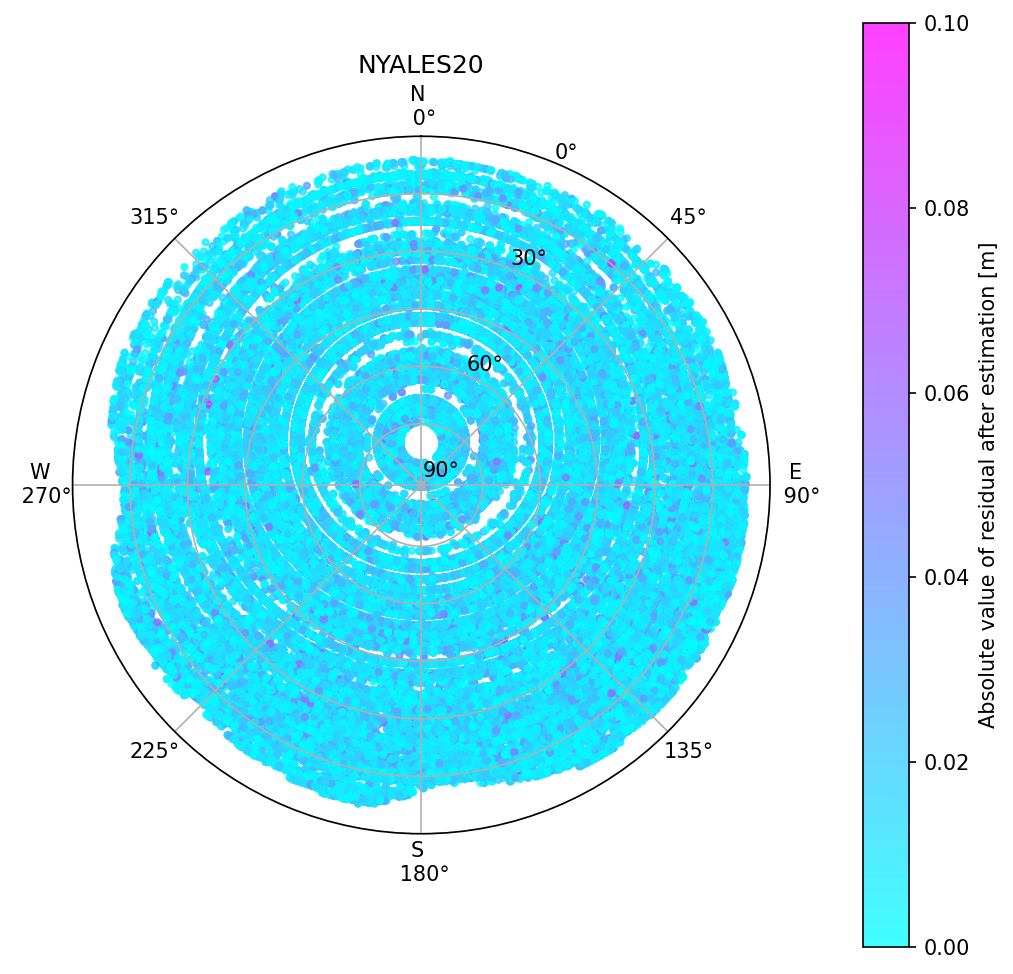
\includegraphics[width=0.5\linewidth]{fig/Skyplot_NYALES20_2020-01-01_2024-04-01_random}} %\\
    % Sky plot NYALE13S - random
	\subfloat[\textcolor{black}{NYALE13S}.\label{fig:sky_random-2}]
      {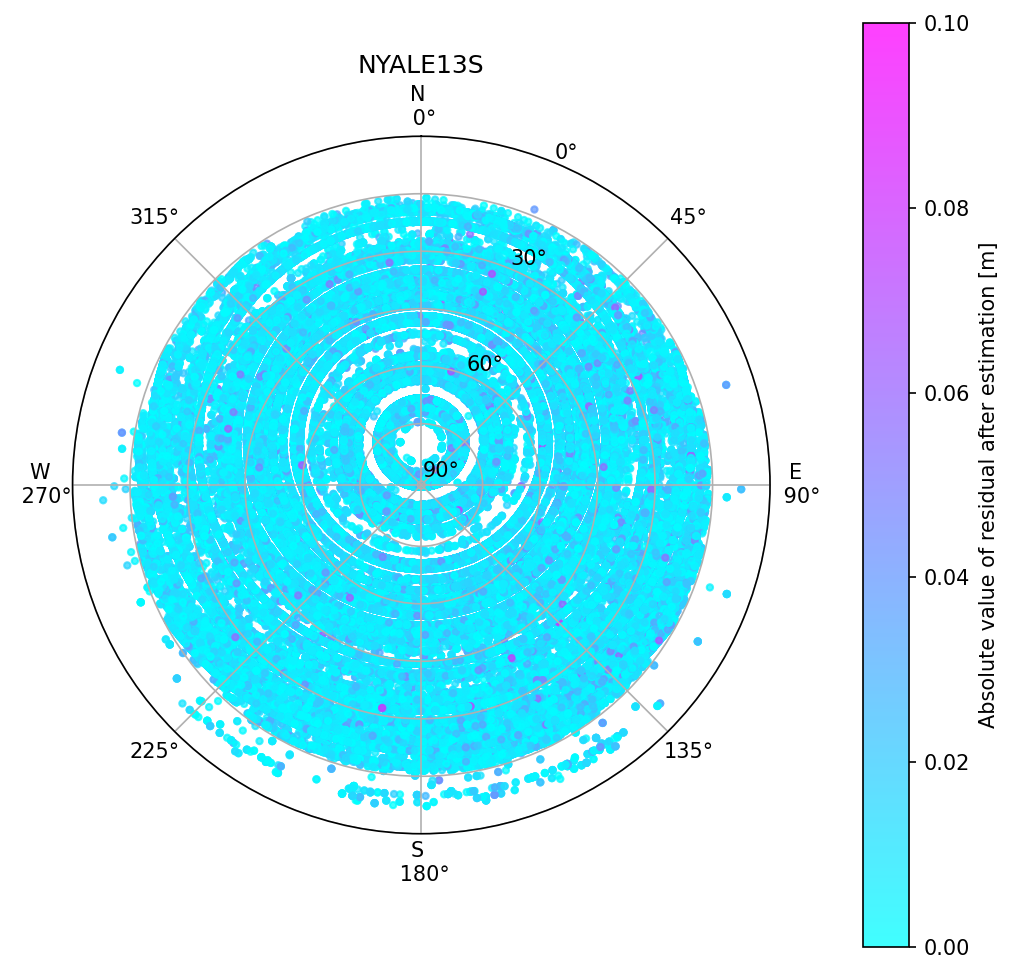
\includegraphics[width=0.5\linewidth]{fig/Skyplot_NYALE13S_2020-01-01_2024-04-01_random}} \\
    % Sky plot WETTZELL - random
	\subfloat[\textcolor{black}{WETTZELL}.\label{fig:sky_random-3}]
      {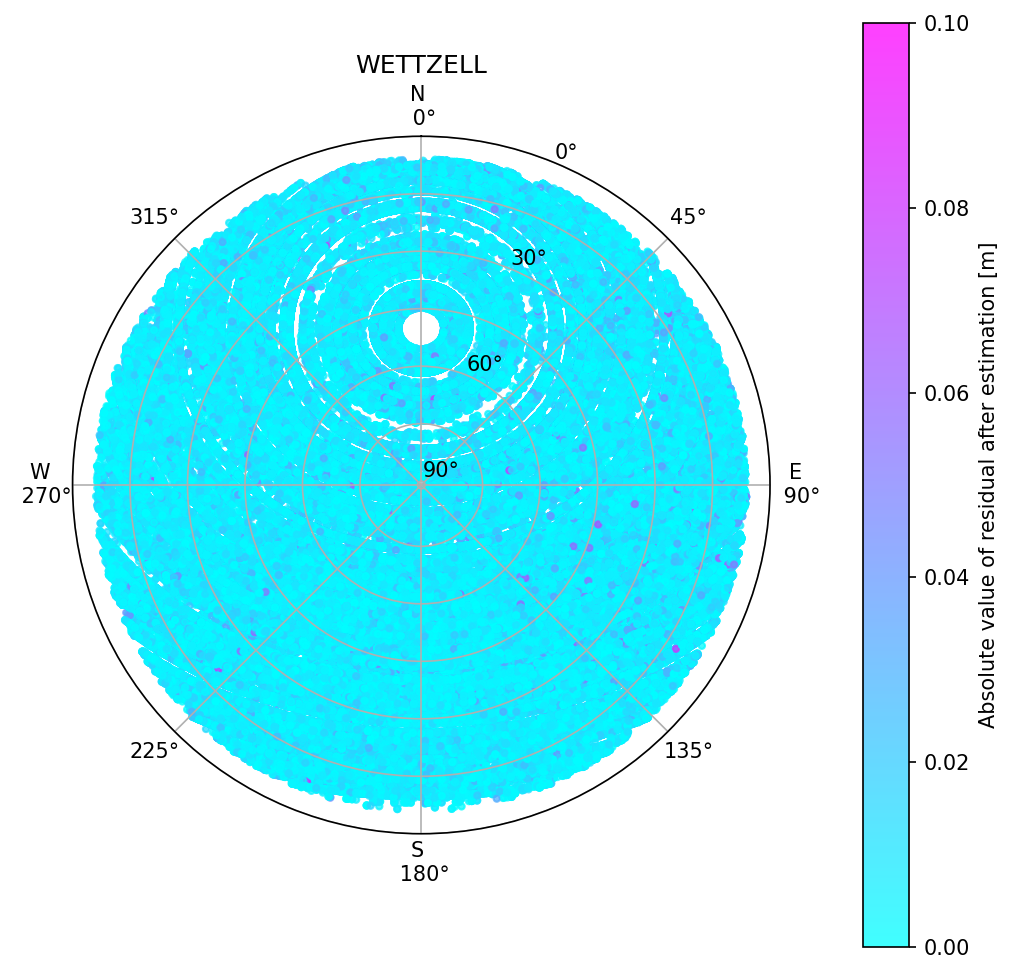
\includegraphics[width=0.5\linewidth]{fig/Skyplot_WETTZELL_2020-01-01_2024-04-01_random}} %\\
    % Sky plot WETTZ13N - random
	\subfloat[\textcolor{black}{WETTZ13N}.\label{fig:sky_random-4}]
      {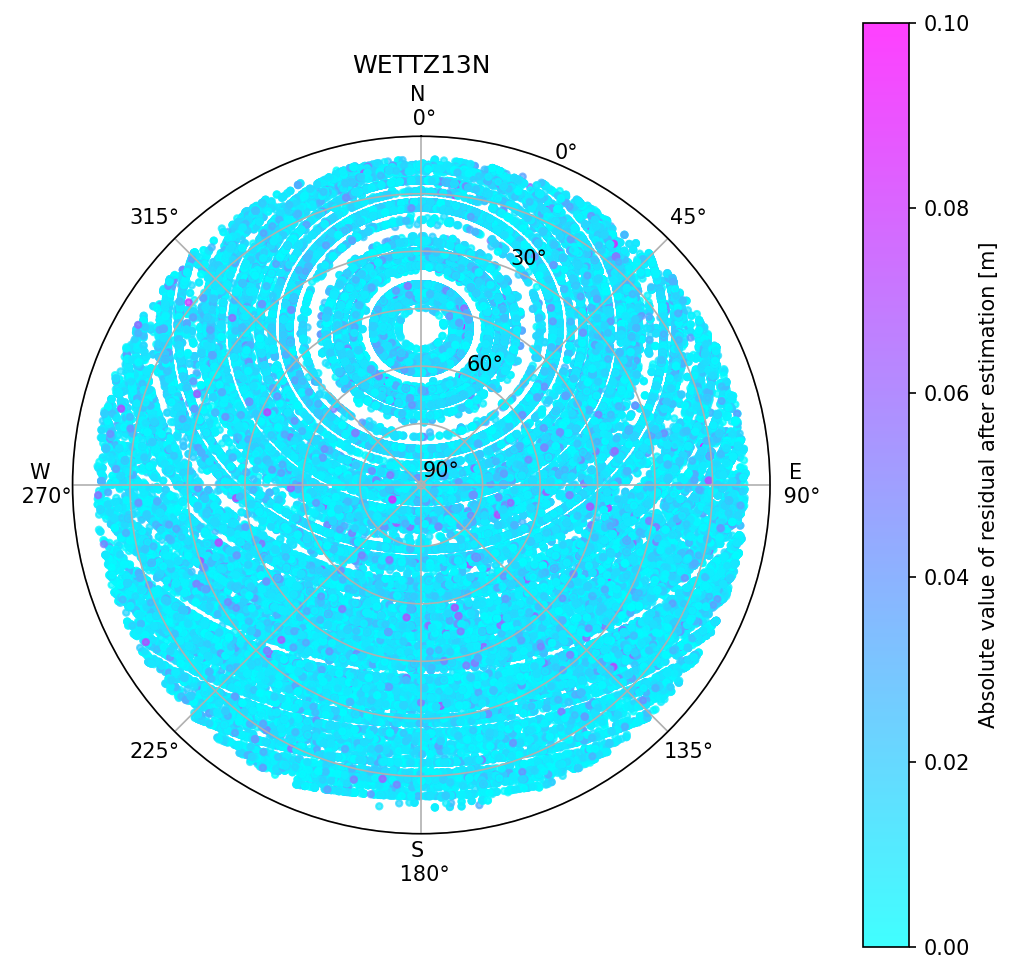
\includegraphics[width=0.5\linewidth]{fig/Skyplot_WETTZ13N_2020-01-01_2024-04-01_random}} \\
    \caption{Accumulated sky plots of the four stations NYALES20 (\ref{fig:sky_random-1}), NYALE13S (\ref{fig:sky_random-2}), WETTZELL (\ref{fig:sky_random-3}) and WETTZ13N (\ref{fig:sky_random-4})
     where 20\% of the
    observations are discarded randomly. The color represents the residual of each observation after estimation. Darker color means higher residuals. The colors may be useful to see if there is a problem in any particular direction.}
	\label{fig:sky_random}
\end{figure}

%nyales: Number of observations total: 2499489
%nyales: Number of observations total for WETTZELL: 528880
%nyales: Number of observations total for WETTZ13N: 173271
%nyales: Number of observations total for NYALE13S: 304603
%nyales: Number of observations total for NYALE13N: 53490
%nyales: Number of observations total for NYALES20: 253821
% nyales = [2499489, 528880, 173271, 304603, 53490, 253821]

%elev15: Number of observations total: 1962340
%elev15: Number of observations total for WETTZELL: 408414
%elev15: Number of observations total for WETTZ13N: 135297
%elev15: Number of observations total for NYALE13S: 269725
%elev15: Number of observations total for NYALE13N: 47672
%elev15: Number of observations total for NYALES20: 203801
%elev15 = [1962340, 408414, 135297, 269725, 47672, 203801]

%random: Number of observations total: 1995716
%random: Number of observations total for WETTZELL: 422149
%random: Number of observations total for WETTZ13N: 138289
%random: Number of observations total for NYALE13S: 243786
%random: Number of observations total for NYALE13N: 42727
%random: Number of observations total for NYALES20: 202504
%random = [1995716, 422149, 138289, 243786, 42727, 202504]

% nyales - elev15 = [537149, 120466,  37974,  34878,   5818,  50020]
% (nyales - elev15)/nyales = [0.21490353, 0.22777568, 0.21915958, 0.11450314, 0.10876799, 0.19706801]
% rounded: [21.5%, 22.7%, 21.9%, 11.5%, 10.9%, 19.7%]
% 
% nyales - random = [503773, 106731,  34982,  60817,  10763,  51317]
% (nyales - random)/nyales = [0.2015504 , 0.2018057 , 0.20189183, 0.19965989, 0.20121518, 0.20217791]
% rounded: [20.2%, 20.2%, 20.2%, 20.0%, 20.1%, 20.2%]

\begin{table}[t]
\captionsetup{labelfont={color=black}}
	\begin{tabularx}{\linewidth}{X|r|r|r|r|r|r|r}
	Station      & Num obs   & Num obs    & Num obs & \multicolumn{2}{r|}{Diff (0$^\circ$-15$^\circ$)} & \multicolumn{2}{r}{Diff (0-random)} \\
	             & 0$^\circ$ & 15$^\circ$ & random  & abs & rel & abs & rel\\
	\hline
	All stations & 2499489   & 1962340    & 1995716 & 537149 & 21\% & 503773 & 20\% \\
	NYALES20     & 253821    & 203801     & 202504  & 120466 & 20\% & 51317  & 20\% \\
	NYALE13S     & 304603    & 269725     & 243786  & 37974  & 11\% & 60817  & 20\% \\
	WETTZELL     & 528880    & 408414     & 422149  & 34878  & 23\% & 106731 & 20\% \\
	WETTZ13N     & 173271    & 135297     & 138289  & 50020  & 22\% & 34982  & 20\%  \\
	\hline
	\end{tabularx}
\caption{{Number of observations for all stations in total and for the specific stations NYALES20, NYALE13S, WETTZELL and WETTZ13N for the three scenarios.
	Column 5 and 6 shows the absolute and relative difference between the first and the second scenario and column 7 and 8 shows the absolute and relative
	difference between the first and the third scenario. }}
\label{tab:num_obs}
\end{table}



\begin{figure}
\centering
\addtocounter{figure}{1}
    % Baseline lengths NYALE13S/NYALES20 - cut off 0 degrees
	\subfloat[\textcolor{black}{NYALE13S/NYALES20 - elevation cut off: $0^{\circ}$}.\label{fig:bl_nsny-1}]
      {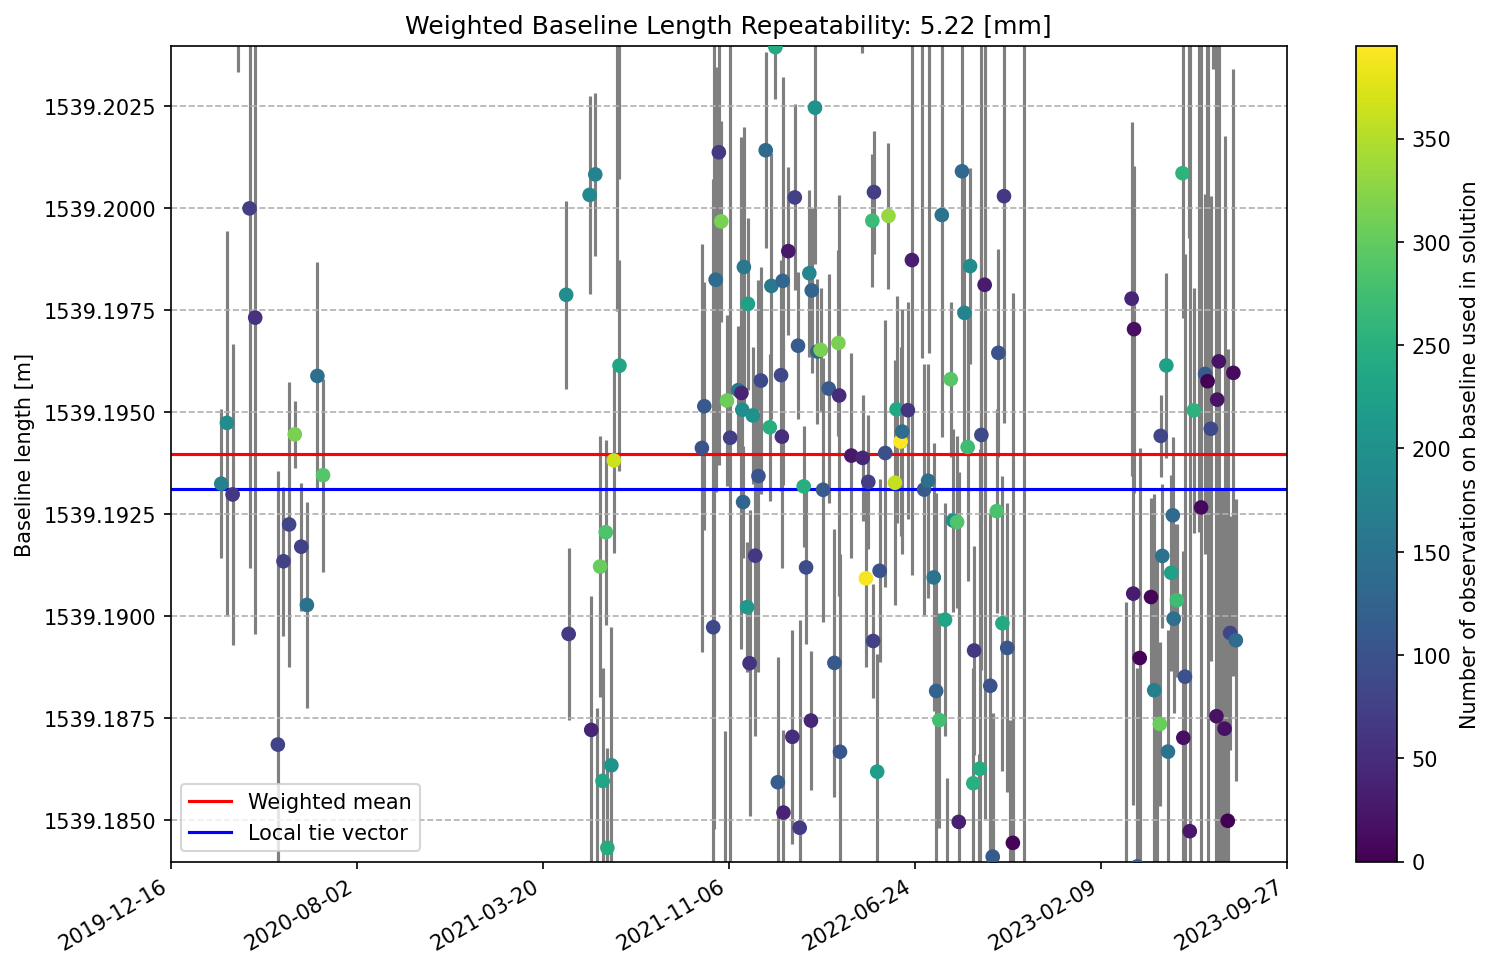
\includegraphics[width=0.9\linewidth]{fig/Baseline_NYALES20_NYALE13S_nyales}} \\
    % Baseline lengths NYALE13S/NYALES20 - cut off 15 degrees
	\subfloat[\textcolor{black}{NYALE13S/NYALES20 - elevation cut off: $15^{\circ}$}.\label{fig:bl_nsny-2}]
      {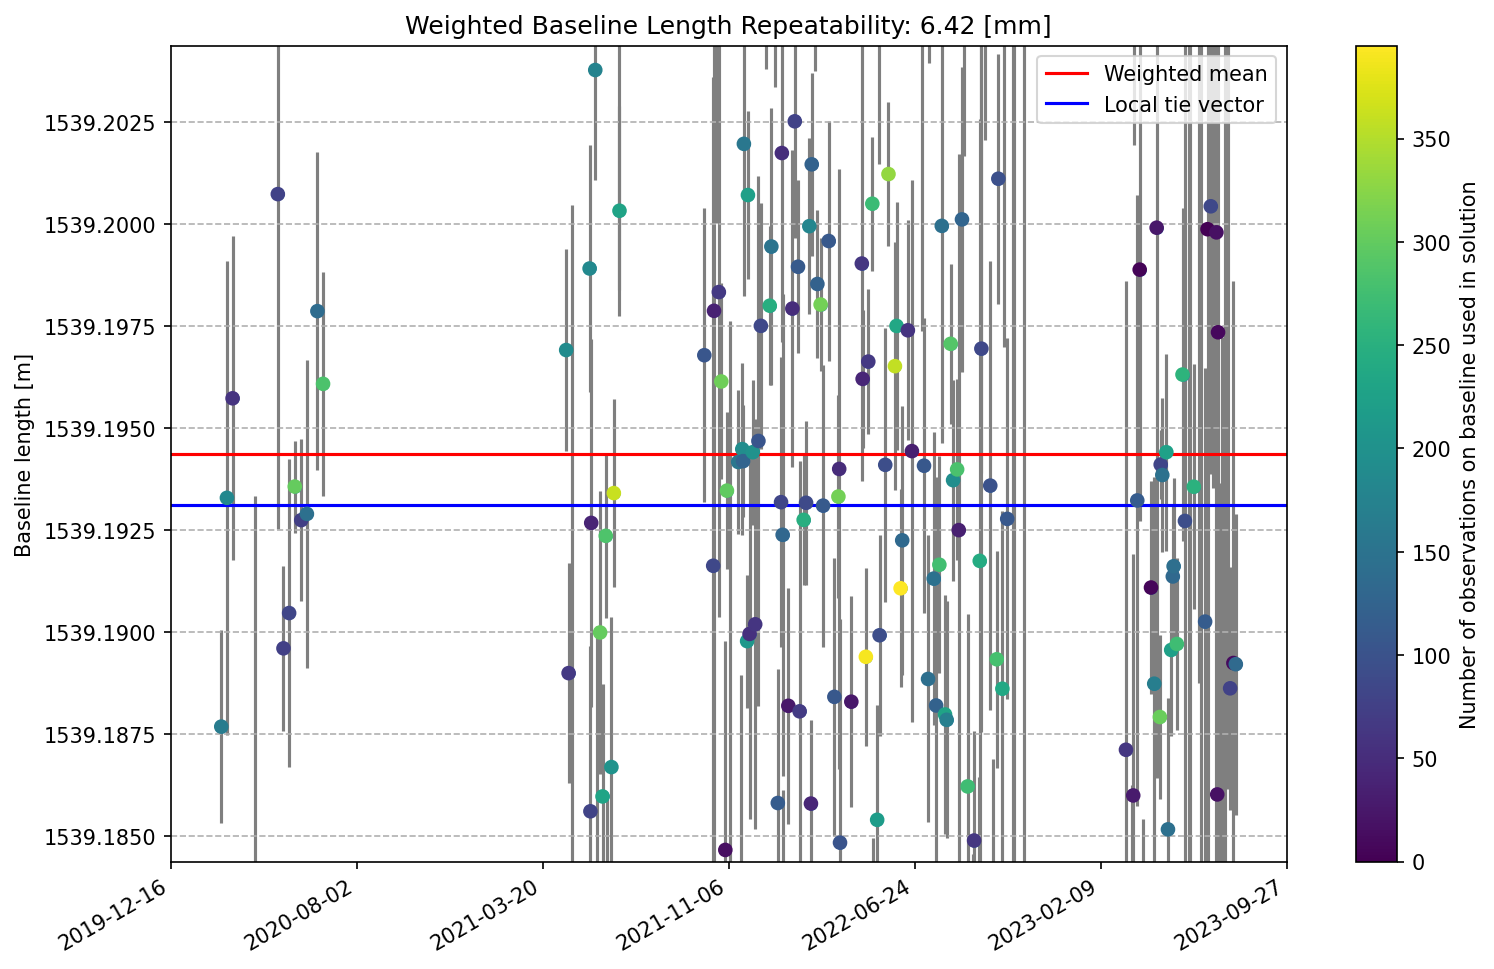
\includegraphics[width=0.9\linewidth]{fig/Baseline_NYALES20_NYALE13S_elev15}} \\
\end{figure}
\begin{figure}\ContinuedFloat
    % Baseline lengths NYALE13S/NYALES20 - random
	\subfloat[\textcolor{black}{NYALE13S/NYALES20 - random}.\label{fig:bl_nsny-3}]
      {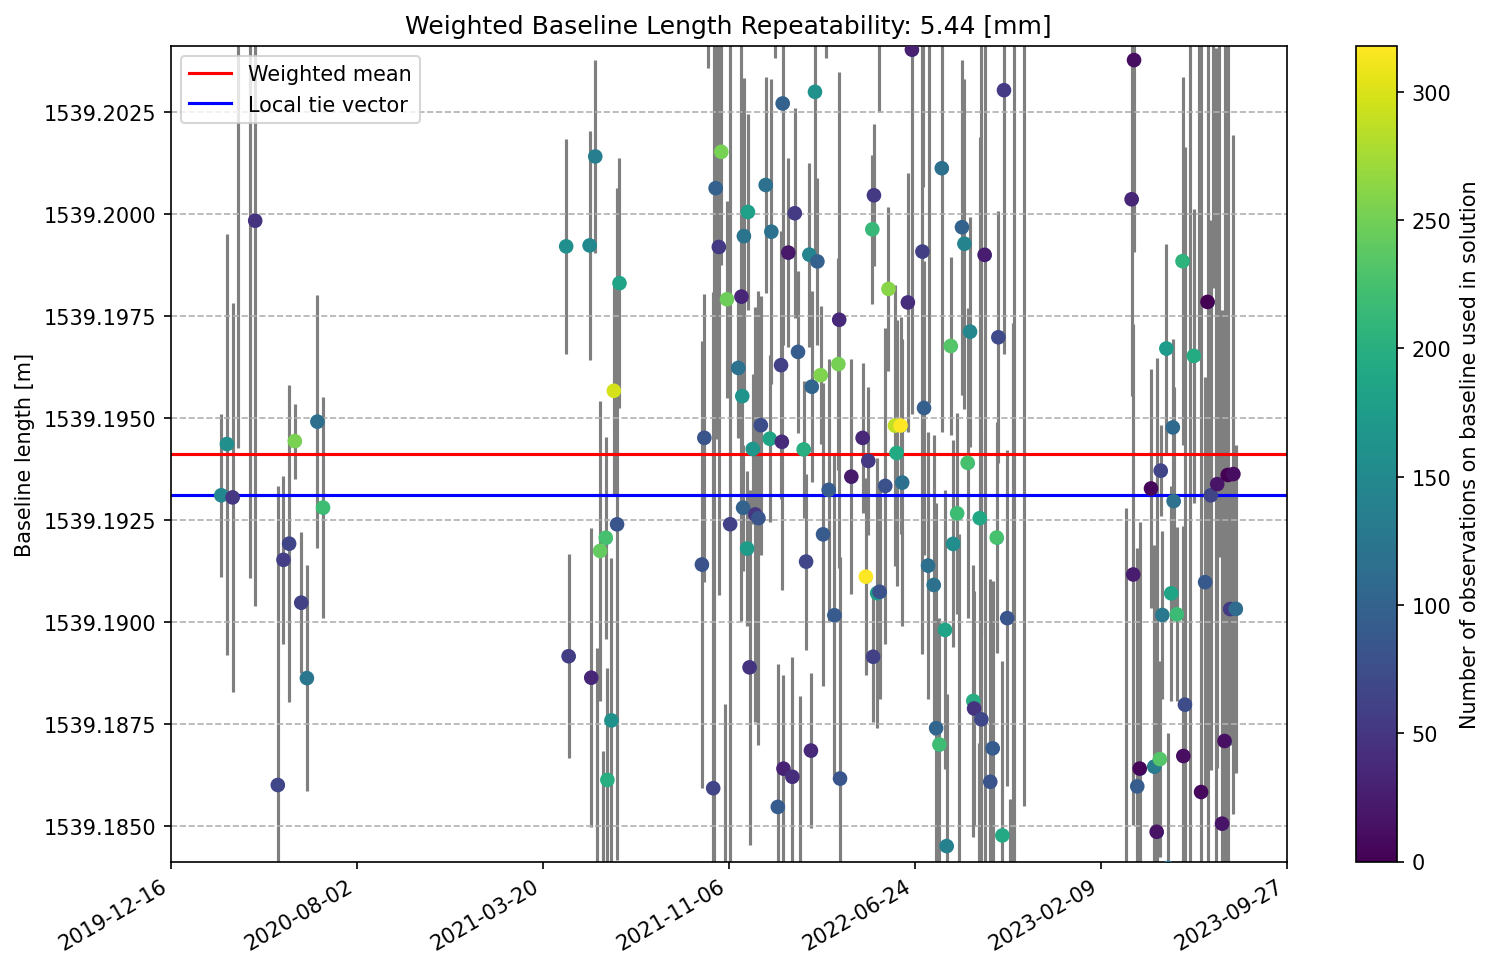
\includegraphics[width=0.9\linewidth]{fig/Baseline_NYALES20_NYALE13S_random}} \\
    \caption{Estimated baseline length of the NYALES20/NYALE13S baseline with different elevation cut off angles. The first plot (\ref{fig:bl_nsny-1}) uses an
    elevation cut off angle of zero degrees and the second plot (\ref{fig:bl_nsny-2}) uses an elevation cut of angle of 15 degrees. The third plot (\ref{fig:bl_nsny-3})
    uses an elevation cut off angle of zero degrees but has discarded 20\% of the observations randomly.}
	\label{fig:bl_nsny}
\end{figure}

\begin{figure}
\centering
\addtocounter{figure}{1}
    % Baseline lengths WETTZELL/WETTZ13N - cut off 0 degrees
	\subfloat[\textcolor{black}{WETTZELL/WETTZ13N - elevation cut off: $0^{\circ}$}.\label{fig:bl_wzwn-1}]
      {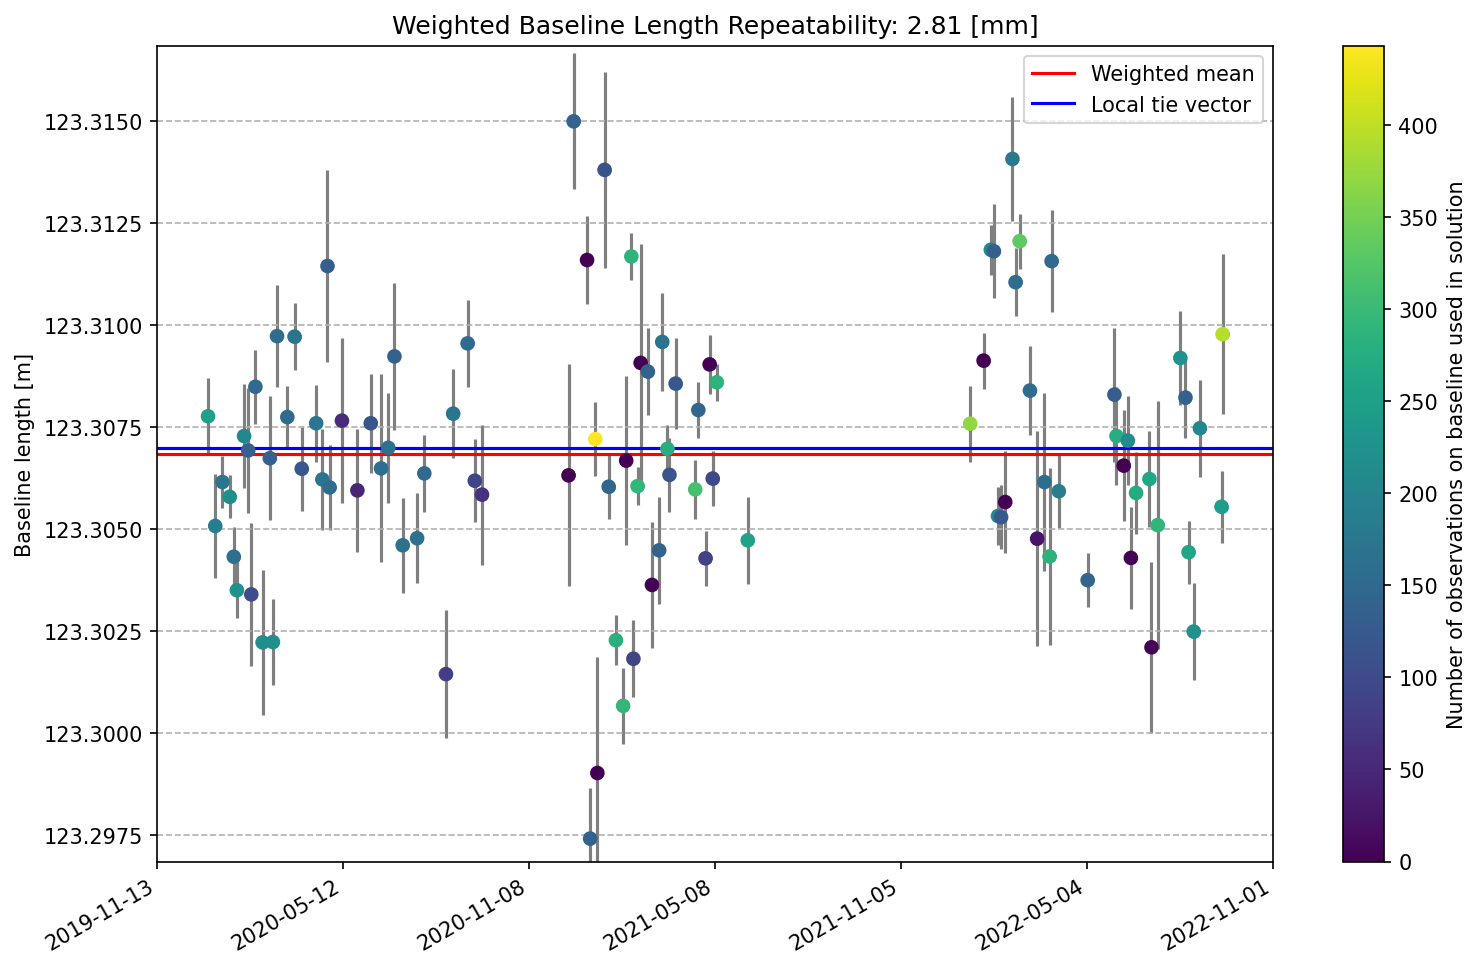
\includegraphics[width=0.9\linewidth]{fig/Baseline_WETTZELL_WETTZ13N_nyales}} \\
    % Baseline lengths WETTZELL/WETTZ13N - cut off 15 degrees
	\subfloat[\textcolor{black}{WETTZELL/WETTZ13N - elevation cut off: $15^{\circ}$}.\label{fig:bl_wzwn-2}]
      {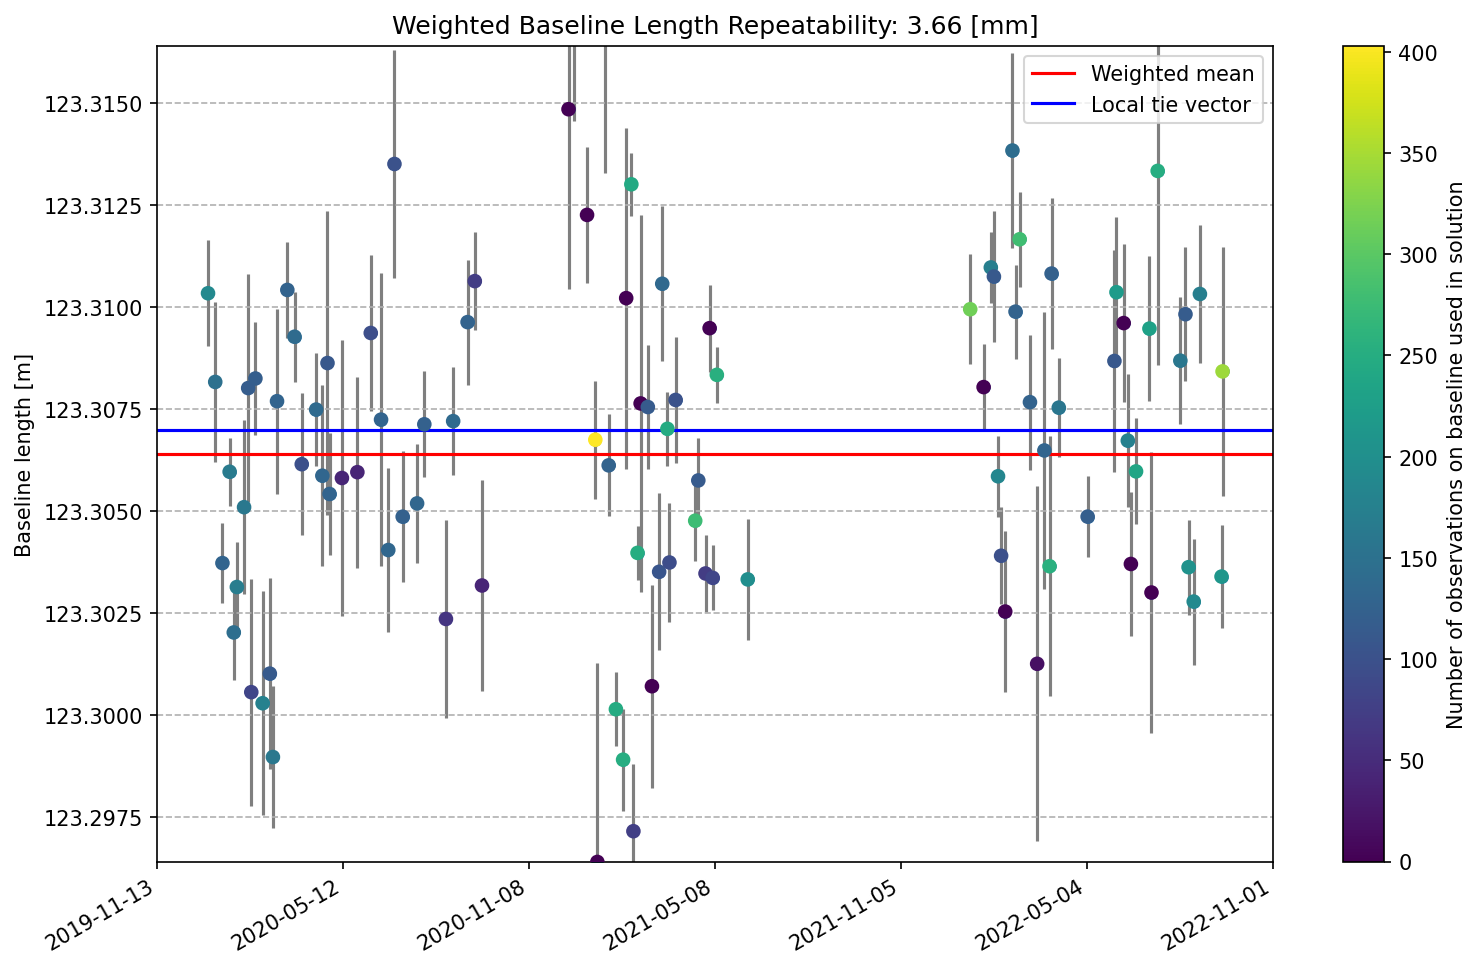
\includegraphics[width=0.9\linewidth]{fig/Baseline_WETTZELL_WETTZ13N_elev15}} \\
\end{figure}
\begin{figure}\ContinuedFloat
    % Baseline lengths WETTZELL/WETTZ13N - random
	\subfloat[\textcolor{black}{WETTZELL/WETTZ13N - random}.\label{fig:bl_wzwn-3}]
      {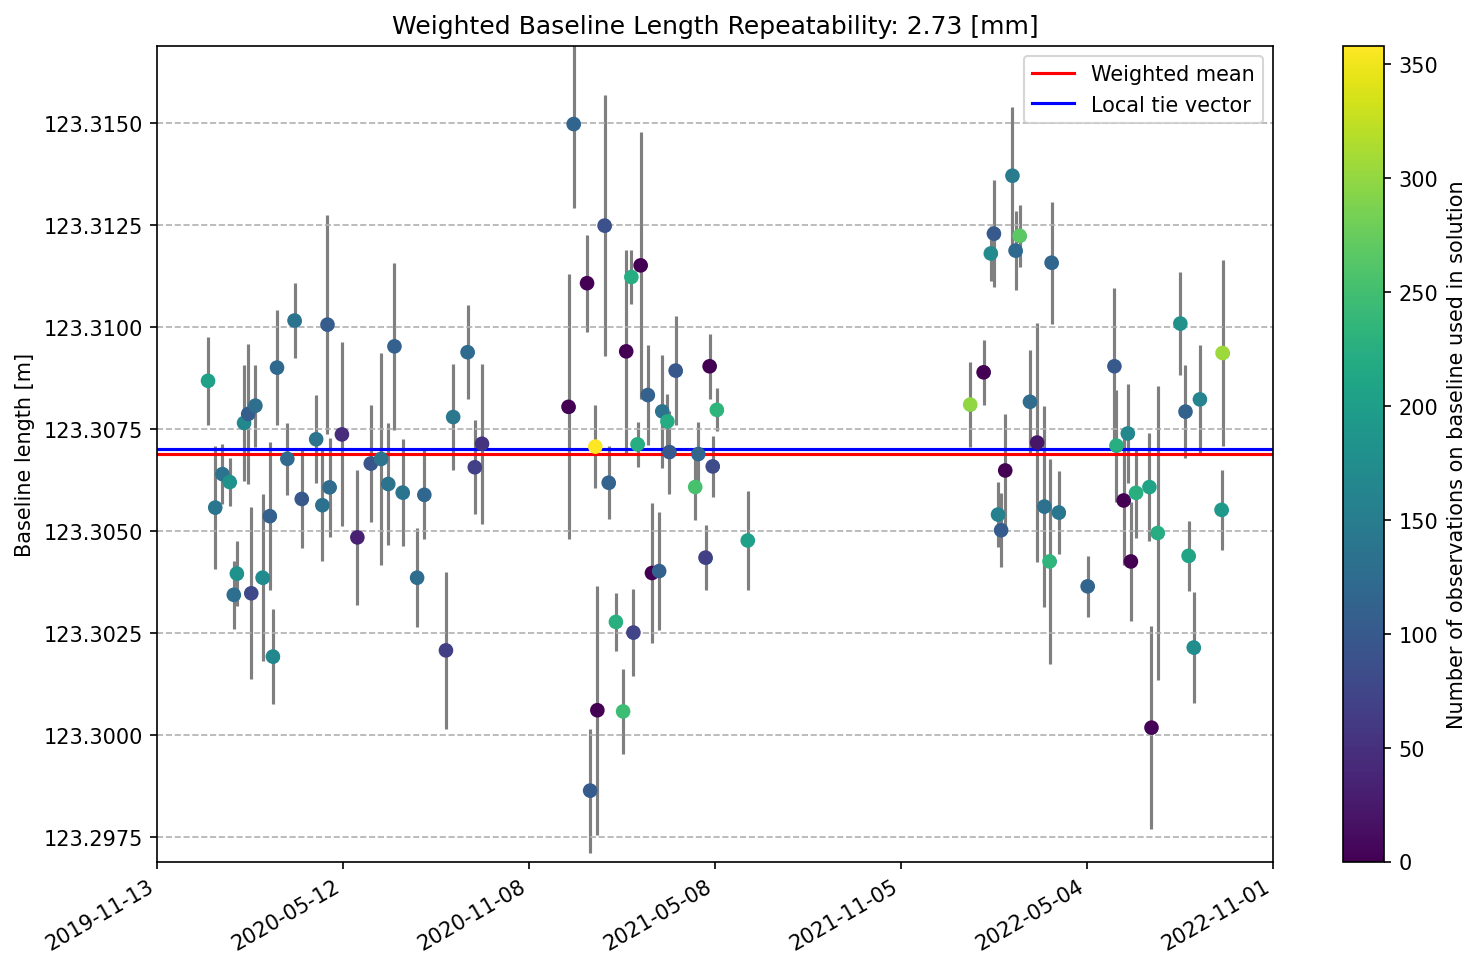
\includegraphics[width=0.9\linewidth]{fig/Baseline_WETTZELL_WETTZ13N_random}} \\
    \caption{Estimated baseline length of the WETTZELL/WETTZ13N baseline with different elevation cut off angles. The first plot (\ref{fig:bl_wzwn-1}) uses an
    elevation cut off angle of zero degrees and the second plot (\ref{fig:bl_wzwn-2}) uses an elevation cut of angle of 15 degrees. The third plot (\ref{fig:bl_wzwn-3})
    uses an elevation cut off angle of zero degrees but has discarded 20\% of the observations randomly.}
	\label{fig:bl_wzwn}
\end{figure}

%This is the results for the NYALES20/NYALE13S baseline:
%  
%Elevation cut off: 0 degrees (default)
%Weighted mean:  1539.1940 [m], Local tie offset:   0.88 [mm]
%Weighted blr (using weighted mean):   5.22 [mm]
%
%Elevation cut off: 15 degrees
%Weighted mean:  1539.1944 [m], Local tie offset:   1.26 [mm]
%Weighted blr (using weighted mean):   6.42 [mm]
%
%random: Weighted mean:  1539.1941 [m], Local tie offset:   1.02 [mm]
%random: Weighted blr (using weighted mean):   5.44 [mm]


%WETTZELL/WETTZ13N:
%
%Elevation cut off: 0 degrees (default)
%Weighted mean:  123.3069 [m], Local tie offset:  -0.14 [mm]
%Weighted blr (using weighted mean):   2.81 [mm]
%
%Elevation cut off: 15 degrees
%elev15: Weighted mean:  123.3064 [m], Local tie offset:  -0.58 [mm]
%elev15: Weighted blr (using weighted mean):   3.66 [mm]

%random: Weighted mean:  123.3069 [m], Local tie offset:  -0.10 [mm]
%random: Weighted blr (using weighted mean):   2.73 [mm]

\begin{table}[t]
\captionsetup{labelfont={color=black}}
	\begin{tabularx}{\linewidth}{X|r|r|r|r}
	Baseline & Scenario & WBL & WBLR & dL \\
	\hline
	NYALE13S/NYALES20 & {0$^\circ$}  & 1539.1940 m & 5.22 mm &  0.88 mm \\
	NYALE13S/NYALES20 & {15$^\circ$} & 1539.1944 m & 6.42 mm &  1.26 mm \\
	NYALE13S/NYALES20 & random       & 1539.1941 m & 5.44 mm &  1.02 mm \\
	WETTZELL/WETTZ13N & {0$^\circ$}  &  123.3069 m & 2.81 mm & -0.14 mm \\
	WETTZELL/WETTZ13N & {15$^\circ$} &  123.3064 m & 3.66 mm & -0.58 mm \\
	WETTZELL/WETTZ13N & random       &  123.3069 m & 2.73 mm & -0.10 mm \\
	\hline
	\end{tabularx}
\caption{{Weighted baseline length (WBL), weighted baseline length repeatability (WBLR) and difference 
between weighted baseline length and local tie vector (dL) for the different baselines.
}}
\label{tab:baselines}
\end{table}

\section{Conclusions and future work}
The results indicate that the performance of NYALE13S should improve if the elevation mask is lowered. This must be done in a safe manner to avoid destroying the LNAs. The elevation mask must therefore be different for different azimuth angles. The same should apply for NYALE13N. NYALE13S and NYALE13N will occasionally observe in the same session and even more often when both stations have installed a VGOS receiver. The performance of this local baseline should be monitored in the future as the NYALES20 antenna no longer exist. 

\newpage
\bibliographystyle{../../where}
\bibliography{../../where}

\end{document}
